\documentclass[11pt]{article}
\usepackage[margin=1in]{geometry}
\usepackage{amsmath,amssymb}
\usepackage{booktabs,array,tabularx}
\usepackage{graphicx}
\usepackage[round]{natbib}
\usepackage[font=small,labelfont=bf]{caption}
\usepackage{microtype}
\usepackage{placeins}
\usepackage[colorlinks=true,linkcolor=blue,citecolor=blue,urlcolor=blue]{hyperref}
\hypersetup{pdftitle={Mixed-model association under population structure},pdfauthor={mixmogam contributors}}
\newcommand{\y}{\mathbf{y}}
\newcommand{\z}{\mathbf{z}}
\newcommand{\w}{\mathbf{w}}
\newcommand{\K}{\mathbf{K}}
\newcommand{\X}{\mathbf{X}}
\newcommand{\V}{\mathbf{V}}
\newcommand{\U}{\mathbf{U}}
\newcommand{\I}{\mathbf{I}}
\newcommand{\Hm}{\mathbf{H}}
\newcommand{\Pm}{\mathbf{P}}
\newcommand{\lgc}{\lambda_{\mathrm{GC}}}
\newcommand{\E}{\mathbb{E}}
\newcommand{\Var}{\operatorname{Var}}
\newcommand{\tr}{\operatorname{tr}}
\newcommand{\diag}{\operatorname{diag}}
\newcommand{\code}[1]{\texttt{#1}}
\makeatletter
\newcommand{\tabinput}[1]{\@@input #1 }
\makeatother
\setlength{\emergencystretch}{1em}
\renewcommand{\topfraction}{.9}
\renewcommand{\bottomfraction}{.8}
\renewcommand{\textfraction}{.1}
\renewcommand{\floatpagefraction}{.8}

\title{Mixed-model association under population structure:\\
numerical foundations, calibration diagnostics\\
and research directions for mixmogam}
\author{mixmogam contributors}
\date{3 October 2026\\\small Research report for version 2.0.0.dev1}

\begin{document}
\maketitle

\begin{abstract}
Mixed-model association combines a model of genetic background with a
numerical approximation and a reference distribution for testing. These
three parts require separate validation. We describe the revised
mixmogam package and examine how population structure exposes their
differences. The package provides dense and streaming Gaussian
mixed-model analyses, leave-one-chromosome-out (LOCO) scans, and
experimental two-step approximations. We derive the dependence of the
association denominator on a variant's orientation in the kinship
spectrum and show why calibration averaged over variants can conceal
opposing errors. In a new conditional experiment with known covariance,
256 samples, and 970 held-out audit variants, scalar calibration gives
an overall rejection probability of 1.00\% at a nominal 1\% threshold
under moderate frequency dispersion, but 1.19\% and 0.73\% in the lowest
and highest structure-loading quintiles. A rank-four spectral correction
reduces that spread to 1.010\% and 1.005\%. Analytic probabilities agree
with simulations across 2,000 independent phenotype replicates.
These results establish a mechanism under a controlled Gaussian null;
they do not validate estimated-covariance scans or reference GWAS
programs. We reassess historical simulations, separate environmental
mean misspecification from denominator error, and withdraw an external
comparison compromised by genotype encoding. A reproducible research
agenda prioritizes matched-input benchmarks, independent calibration
audits, error-controlled spectral approximations, and validation under
realistic ancestry, relatedness, and genetic architectures.
\end{abstract}

\section{Introduction}

A mixed-model association test asks whether a candidate variant explains
phenotypic variation beyond specified covariates and a model of genetic
background. Its appeal is that the same relationship matrix can describe
close relatives, cryptic relatedness, and broad population structure.
Early efficient implementations made this approach practical in model
organisms and human association studies
\citep{kang2008,kang2010,lippert2011,zhou2012}. The resulting test is
nevertheless conditional on assumptions about the phenotype mean, the
background covariance, and the way nuisance parameters are fitted. A
precise matrix calculation cannot repair a misspecified mean, and a
well-fitted prediction model does not by itself supply a valid association
test.

The computational problem has changed with cohort size. Dense methods
factorize an $n\times n$ covariance matrix and reuse the factorization
across variants. Large-cohort methods instead use iterative fitting,
whole-genome prediction, and approximate association statistics.
BOLT-LMM combines mixed-model association with a mixture prior on marker
effects \citep{loh2015}; REGENIE constructs whole-genome predictions
through successive ridge regressions \citep{mbatchou2021}; and newer
approaches include LDAK-KVIK \citep{hof2025} and the variational method
Quickdraws \citep{loya2025}. These programs have distinct fitting and
testing procedures. A claim about one denominator approximation should
therefore be evaluated at the level of that approximation, rather than
assigned to all methods with a two-step workflow.

Two statistical choices cut across these computational designs. First,
a candidate variant and its correlated neighbours can contribute to the
random-effect predictor against which they are tested. This proximal
contamination can reduce power; excluding the candidate chromosome or
region changes that overlap \citep{listgarten2012,yang2014}. Second,
ancestry can influence both allele frequencies and environmental
exposures. Modelling genetic covariance and adjusting the phenotype mean
with principal components (PCs) address different parts of this problem
\citep{price2006,vilhjalmsson2013}. Neither chromosome exclusion nor
covariance modelling makes environmental confounding disappear as a
matter of algebra.

This report focuses on a third, more specific issue: the denominator of
an association statistic depends on how the tested variant aligns with
the covariance eigenvectors. Replacing that denominator by a scalar
multiple of the variant norm can work well when this alignment has
little effect. Under structure, a satisfactory average can instead hide
inflation in one class of variants and deflation in another. The relevant
object is the conditional rejection probability for a variant, or a
prespecified class of variants, under a stated null model. A single
genome-wide median is an incomplete diagnostic of that object.

mixmogam offers a useful setting for studying these distinctions because
dense and streaming calculations share genotype handling and several
model components. Its earlier work included multi-locus mixed-model
association \citep{segura2012}; the current engine also supplies LOCO and
experimental two-step analyses. The present contribution is a methods
and software investigation, not a competitive benchmark establishing a
new best-performing GWAS program. We provide the mathematical contracts
needed to interpret its outputs, a new known-covariance experiment with
a disjoint set of audit variants, and a critical reading of archived
simulations. We then formulate research questions that can distinguish
a useful general method from an approximation that works only in a
favourable example.

The evidence has three levels. Current software checks assess specified
numerical and data-handling contracts. The new experiment isolates
calibration geometry under a deliberately simple null. Historical
simulations motivate broader questions but predate the scientific
correctness review. Table~\ref{tab:evidence} records these boundaries;
they apply throughout the report.

\begin{table}[htbp]
\centering\small
\caption{Evidence used in this revision and the inference it supports.
Historical archives are preserved, not silently reclassified as results
from the corrected package.}
\label{tab:evidence}
\begin{tabularx}{\textwidth}{@{}>{\raggedright\arraybackslash}p{.23\textwidth}>{\raggedright\arraybackslash}X>{\raggedright\arraybackslash}X@{}}
\toprule
Evidence & Established here & Remaining boundary \\
\midrule
Current review, 2.0.0.dev1 & Regression and independent numerical checks;
117 local tests passed; installed-artifact checks & Test coverage does
not establish population calibration. \\
New denominator experiment & Analytic conditional rejection probabilities,
checked by independent phenotype replicates & Known Gaussian covariance,
small fixed genotype panels, exact leading eigenvectors. \\
Archived simulations & Descriptive patterns under the recorded historical
implementation & New input handling and fitting changes need fresh
end-to-end runs. \\
Archived external comparison & A provenance failure was identified:
incorrect PLINK export encoding & External-program calibration, agreement,
and superiority claims are withdrawn pending a matched-input rerun. \\
\bottomrule
\end{tabularx}
\end{table}

\section{Statistical and computational methods}
\label{sec:methods}

\subsection{Data, estimand, and relationship matrix}

Let $\y\in\mathbb{R}^n$ be a quantitative phenotype, $\X$ a full-rank
$n\times p$ covariate matrix including an intercept, and $\z_j$ a
centered candidate genotype. The coefficient of interest, $\alpha_j$,
is the fixed effect in a specified marginal mixed model after integrating
out the random genetic background. It is not automatically a direct
causal effect: linkage disequilibrium (LD), omitted exposures, and the
choice of background model affect its interpretation. The null is
$H_{0j}:\alpha_j=0$ under that model. A variant without a designated
large QTL effect need not satisfy this null if a simulated polygenic
background still assigns it an effect.

The relationship matrix summarizes the covariance induced by a
polygenic marker model \citep{yang2010}. For the unweighted matrix,
mixmogam centers each marker by
its mean among called samples and divides by its empirical standard
deviation among those samples. Missing calls become zero after this
transformation, corresponding to mean imputation. Write the resulting
background matrix as $\mathbf Z$, with $M$ retained polymorphic markers.
Its raw relationship matrix and a weighted extension are
\begin{equation}
 \K_0=\frac{1}{M}\mathbf Z\mathbf Z^\top,
 \qquad
 \K_w=\frac{\sum_{j=1}^{M} w_j\z_j\z_j^\top}{\sum_{j=1}^{M}w_j},
 \quad w_j\geq0,\quad \sum_j w_j>0.
 \label{eq:grm}
\end{equation}
Empirical-standard-deviation scaling differs from using the
Hardy--Weinberg variance $2f_j(1-f_j)$; these definitions should not be
interchanged in a reference comparison. The optional kinship rescaling
subtracts the mean off-diagonal entry from every entry and divides by
the resulting mean diagonal. An intercept absorbs the constant-matrix
shift in the residual subspace. The raw, unrescaled matrix is used in
the new experiment in Section~\ref{sec:newdesign}.

The current input contract is diploid hard calls $0,1,2$, with $-1$ for
missing values. It is not a continuous-dosage interface. Minor allele
count is measured in allele copies. Sample identifiers must align
uniquely; silently intersecting phenotype and genotype rows in different
orders changes the scientific problem. PLINK effect-allele orientation,
missingness, and identifier preservation are consequently part of the
statistical contract, not merely file-format details.

\subsection{Gaussian model, variance fitting, and chromosome exclusion}

For a candidate in chromosome group $g$, the working model is
\begin{equation}
 \y=\X\boldsymbol\beta+\z_j\alpha_j+\mathbf u+\mathbf e,
 \quad \mathbf u\sim N(0,\sigma_g^2\K_{-g}),\quad
 \mathbf e\sim N(0,\sigma_e^2\I),\quad \mathbf u\perp\mathbf e.
 \label{eq:model}
\end{equation}
Here $\K_{-g}$ is constructed without the markers in group $g$.
The subscript on $\sigma_g^2$ denotes genetic variance, not the group
index. With $\delta=\sigma_e^2/\sigma_g^2$, set
$\Hm=\K_{-g}+\delta\I$ and $\V=\sigma_g^2\Hm$.
This parameterization assumes a positive genetic scale; the
zero-genetic-variance limit reduces to a linear model.

The covariance shape is fitted under the null $\alpha_j=0$. For fixed
$\delta$, define the residual precision matrix
\begin{equation}
 \Pm_H=\Hm^{-1}-\Hm^{-1}\X
       (\X^\top\Hm^{-1}\X)^{-1}\X^\top\Hm^{-1}.
 \label{eq:projection}
\end{equation}
Up to constants independent of $\delta$, the profiled restricted
log-likelihood is
\begin{equation}
 \ell_R(\delta)=-\frac12\left\{
 \log|\Hm|+\log|\X^\top\Hm^{-1}\X|
 +(n-p)\log\left(\frac{\y^\top\Pm_H\y}{n-p}\right)\right\}.
 \label{eq:reml}
\end{equation}
Thus $\widehat\sigma_g^2=\y^\top\Pm_H\y/(n-p)$ for REML at the fitted
$\delta$. Maximum likelihood instead uses $n$ and omits the covariate
determinant term. Confusing these objectives changes both the fit and
its interpretation. A phenotype entirely explained by $\X$ has zero
residual variance and is rejected rather than assigned numerical noise
as a variance estimate.

LOCO matrices can be formed by subtracting group-specific cross-products
from the genome-wide sum. The dense implementation refits variance
components for each group; the streaming infinitesimal path uses one
global variance fit and group-specific solves. These are distinct
nuisance-fitting procedures. When chromosome labels are numerous, the
implementation can merge them into a limited number of groups, so the
actual grouping must accompany the results. Exclusion reduces direct
overlap between the tested region and its background predictor; it does
not imply statistical independence across groups or correct an omitted
phenotype mean.

\subsection{What an exact scan makes exact}
\label{sec:exact}

For a fixed covariance shape $\Hm$, let
$U_j=\z_j^\top\Pm_H\y$, $q_j=\z_j^\top\Pm_H\z_j$, and
$S_0=\y^\top\Pm_H\y$. Generalized least squares gives
\begin{equation}
 \widehat\alpha_j=\frac{U_j}{q_j},\qquad
 F_j=\frac{U_j^2/q_j}{(S_0-U_j^2/q_j)/(n-p-1)}.
 \label{eq:f}
\end{equation}
Under a Gaussian null with this \emph{fixed, correct} covariance shape,
$q_j>0$, and positive residual degrees of freedom,
$F_j\sim F_{1,n-p-1}$. In EMMAX-style scans, however, $\delta$ is first
estimated from the phenotype and then held fixed while variants are
tested \citep{kang2010}. The same algebra can be computed accurately,
but the finite-sample reference law is then a plug-in approximation.
Throughout this report, ``exact scan'' refers to the dense calculation
with its fitted covariance, not a guarantee of exact type-I error.

The corresponding known-covariance score test is particularly useful
for analysis. Replace $\Hm$ by the fully specified $\V$ in
Equation~\eqref{eq:projection} to obtain $\Pm_V$. Since
$\Pm_V\V\Pm_V=\Pm_V$, the null statistic satisfies
\begin{equation}
 T_j=\frac{(\z_j^\top\Pm_V\y)^2}{\z_j^\top\Pm_V\z_j}
 \sim\chi^2_1.
 \label{eq:score}
\end{equation}
This conditional result is the reference for the new experiment. It
avoids conflating an approximation to the denominator with uncertainty
in estimated variance components. Variants collinear with the covariates
have zero residual norm and are not estimable.

\subsection{Scalar calibration and its spectral meaning}
\label{sec:scalar}

Work in orthonormal coordinates spanning the complement of $\X$.
Let $R^\top R=\I_d$, $R^\top\X=0$, and $d=n-p$; use
$\widetilde\y=R^\top\y$, $\widetilde\z_j=R^\top\z_j$, and
$\widetilde\K=R^\top\K R$. For the rest of this subsection the tildes
are suppressed. The infinitesimal solve is
$\w=(\K+\delta\I)^{-1}\y$. A retrospective statistic uses
$D_j^{\mathrm{ret}}=(\z_j^\top\z_j/d)\|\w\|^2$ in the denominator
of $(\z_j^\top\w)^2$. The matching prospective denominator is
$D_j^{\mathrm{pro}}=\sigma_g^2 q_j$, where
$q_j=\z_j^\top(\K+\delta\I)^{-1}\z_j$.
A calibration factor averages $D_j^{\mathrm{pro}}/D_j^{\mathrm{ret}}$
over selected markers. A common factor can reproduce the prospective
statistic for all markers only when the relevant ratios are constant.

Write $\K=\U\Lambda\U^\top$ and
$a_{\ell j}=\U_\ell^\top\z_j$. The missing geometry is explicit:
\begin{equation}
 q_j=\sum_{\ell=1}^{d}\frac{a_{\ell j}^2}{\lambda_\ell+\delta},
 \qquad
 \|\z_j\|^2=\sum_{\ell=1}^{d}a_{\ell j}^2.
 \label{eq:spectrum}
\end{equation}
A direction assigned high background variance receives low precision.
Two variants with equal norms can therefore have different $q_j$.
A denominator calibrated to the average may be too small for variants
concentrated in low-variance directions and too large for variants
concentrated in high-variance directions.

For known covariance and a deterministic approximate denominator
$\widehat q_j$, put $r_j=q_j/\widehat q_j$. The consequence is exact:
\begin{equation}
 \widetilde T_j=r_j T_j,\qquad
 \Pr(\widetilde T_j>c_\alpha\mid\mathbf Z)
 =\overline F_{\chi^2_1}\!\left(\frac{c_\alpha}{r_j}\right),
 \quad c_\alpha=F^{-1}_{\chi^2_1}(1-\alpha).
 \label{eq:tail}
\end{equation}
An error that appears modest near the center can matter much more in
the tail. Averaging Equation~\eqref{eq:tail} over a variant group gives
its expected rejection fraction, without assuming variants are
independent. It is a marginal rejection probability, not the
family-wise probability of at least one discovery.

\subsection{A low-rank correction and its current limits}
\label{sec:spectral}

Retaining the leading $k$ eigenpairs and replacing the rest by their mean
$\bar\lambda_{>k}$ gives the approximation
\begin{equation}
 q_j^{(k)}=\sum_{\ell\leq k}\frac{a_{\ell j}^2}{\lambda_\ell+\delta}
 +\frac{\|\z_j\|^2-\sum_{\ell\leq k}a_{\ell j}^2}
       {\bar\lambda_{>k}+\delta},\qquad
 \widehat q_j=c_k q_j^{(k)}.
 \label{eq:spectral}
\end{equation}
The scalar $c_k$ corrects average remaining error; it cannot remove
arbitrary variation in the spectral tail. For a LOCO analysis, each
approximation should target the covariance used by that group's test.
Using a full-genome basis to approximate a different LOCO covariance
requires its own error assessment.

The production implementation computes group-specific bases with
randomized subspace iteration and currently tries widths
64, 128, 256, and 512. It stops when the coefficient of variation of
calibration ratios is at most 3\%, subject to the available dimension.
The calibration markers also determine the scale, so this stopping
criterion is an internal diagnostic. It is not an independent validation
and does not bound the error at genome-wide thresholds. The production
infinitesimal calibration also selects candidate markers using a
phenotype-dependent statistic; this differs from the phenotype-independent
selection in our controlled experiment.

For mixture-prior and elastic-net residuals, an infinitesimal spectral
factor is transferred before further calibration. Once the residual is
a nonlinear, data-adaptive function of $\y$, the proof of
Equation~\eqref{eq:score} no longer supplies its null law. This transfer
is a heuristic. The names ``BOLT-style'' and ``KVIK-style'' below denote
mixmogam implementations inspired by the corresponding methods; they
do not establish equivalence to the reference programs.

\subsection{Environmental mean misspecification}
\label{sec:environment}

Suppose the actual conditional mean includes an omitted exposure vector
$\mathbf d$ with effect $\gamma$:
$\E(\y\mid\mathbf Z,\mathbf d)=\X\boldsymbol\beta+\mathbf d\gamma$.
Even if the covariance $\V$ is known correctly, the numerator in
Equation~\eqref{eq:score} then has mean
$\z_j^\top\Pm_V\mathbf d\gamma$. Its distribution becomes
\begin{equation}
 T_j\sim\chi^2_1(\eta_j),\qquad
 \eta_j=\frac{(\z_j^\top\Pm_V\mathbf d\gamma)^2}
                  {\z_j^\top\Pm_V\z_j}.
 \label{eq:noncentral}
\end{equation}
A kinship matrix can assign large variance to an ancestry direction,
but it does not automatically place an environmental mean shift in
$\X$. Adding covariates that span $\mathbf d$ makes the numerator mean
zero under this model. Estimated PCs may only approximate that span,
and neither the required number of PCs nor a power-preserving adjustment
follows from this identity alone. Reviews of structure and mixed models
place this distinction in a broader setting
\citep{price2010,sul2018,yang2014}.

\subsection{Numerical implementation and ancillary inference}

Dense scans whiten genotype blocks and use matrix products to evaluate
Equation~\eqref{eq:f}. Dense factorization costs $O(n^3)$ time and
$O(n^2)$ storage, with a dense transformation cost of order $n^2m$ for
$m$ tested variants. Streaming methods replace stored kinships by
products with standardized genotype blocks. A product with $r$ right-hand
sides costs order $nMr$ arithmetic; its memory consists of the right-hand
sides, working blocks, and configured caches. Avoiding an $n\times n$
kinship does not mean constant memory: a genotype cache can still
approach the size of the standardized data.

Conjugate gradients supplies covariance solves, and stochastic Lanczos
quadrature estimates likelihood terms for large samples. Both introduce
numerical approximations beyond the statistical model. Association
solves now reject nonconvergence. Variational fits expose incomplete
convergence, and fit caches respect their options and model ownership.
The review also removed an unnecessary LOCO-group axis from temporary
products; Section~\ref{sec:computation} reports the measured allocation
change with its scope.

Several adjacent routines need equally explicit contracts. The genetic
BLUP is $\widehat{\mathbf u}=\K\Hm^{-1}
(\y-\X\widehat{\boldsymbol\beta})$; the genetic scale cancels and must
not be multiplied in a second time. Default permutation inference
operates on orthogonal residual coordinates rather than permuting the
correlated entries of a projected residual vector, following the
underlying distinction developed by \citet{abney2015}. Exact exchangeability
requires the stipulated Gaussian covariance; substituting fitted
variance components still requires calibration checks. Finally, the
normal-approximation Bayes factor requires effect estimates, standard
errors, and an explicit effect-variance prior \citep{wakefield2009}.
It is not a replacement for a joint fine-mapping model. Appendix~\ref{sec:appendix}
gives these identities and their interpretation.

\section{Evaluation design and provenance}
\label{sec:evaluation}

\subsection{New conditional experiment with known covariance}
\label{sec:newdesign}

The new experiment isolates Equation~\eqref{eq:tail}; it does not call
an end-to-end GWAS scan. We generate 256 diploid samples in four equal
populations, with 2,000 background and 1,000 candidate markers. For each
marker, the ancestral frequency $f_j$ is uniform on $[0.1,0.9]$.
Population-specific frequencies are independent draws from
$\operatorname{Beta}(f_j(1/\theta-1),(1-f_j)(1/\theta-1))$ for
$\theta>0$; at $\theta=0$ they all equal $f_j$.
Hard calls are binomial with two trials. The values
$\theta\in\{0,0.05,0.20\}$ control frequency dispersion. We do not
report them as measured $F_{ST}$, whose estimation and interpretation
require a separate definition \citep{bhatia2013}.

Markers are independent conditional on population frequencies and sample
membership. Population structure nevertheless correlates their
sample-level patterns. Monomorphic markers are removed: one background
marker is dropped in the $\theta=0.20$ panel; all 1,000 candidates
remain in every panel. The package's raw relationship matrix is checked
against a direct standardized cross-product. We remove an intercept in
orthonormal residual coordinates, set $\delta=1$ and genetic scale one,
and use a full eigendecomposition to obtain the known covariance.
Direct linear solves and spectral denominators agree to numerical
precision.

Thirty randomly selected candidates calibrate each approximation;
the other 970 are held out for audit. Selection is independent of
phenotype. The scalar denominator is the variant norm times the mean
$q_j/\|\z_j\|^2$ among calibration markers. For the spectral method,
we try $k\in\{4,8,16,32,64,128\}$ and select the first width whose
calibration-ratio coefficient of variation is at most 3\%. All three
panels select $k=4$. These exact leading eigenvectors provide a
favourable test of spectral geometry, not a validation of the production
randomized eigensolver or its width-selection procedure.

Audit variants are divided into quintiles by the share of their squared
norm explained by the top three background eigenvectors. For each method
and quintile we calculate the analytic mean rejection probability at
$\alpha=0.01$ and $5\times10^{-8}$. We also simulate 2,000 independent
Gaussian phenotype replicates per fixed panel and compare the empirical
rejection fraction at 1\% with its analytic value. Methods use the same
phenotypes. Monte Carlo standard errors are calculated from the
replicate-level fractions, retaining correlation among variants within
each replicate. We do not estimate the extreme-tail probability by
counting a handful of simulated exceedances.

The three genotype panels use seeds 20261003--20261005. Consequently,
differences across $\theta$ also include differences among three realized
panels; there are no genotype-replicate confidence intervals. The
analytic result is exact conditional on each realized panel and its
fixed approximation. It is not an estimate of an average over all
possible populations.

\subsection{Historical structure and environmental experiments}
\label{sec:historicaldesign}

The archived structure experiment used 1,300 samples, 20,000 markers,
and five chromosomes, with both unstructured genotypes and a
four-population generator labelled $F_{ST}=0.3$ in the archive. We
retain that label as a generator setting, not a newly estimated
differentiation measure. Six phenotype replicates shared each genotype
panel. Genetic signal was generated outside the last chromosome from
a polygenic component of variance share 0.4 and ten large QTLs of
variance share 0.1. The last chromosome has no generating marker
effects, making it useful for a null-chromosome diagnostic. Sparse QTLs,
realized cross-chromosome correlations, and variance estimation mean
that this is not the known-Gaussian-covariance experiment above.
Loading quintiles use the leading ten kinship eigenvectors.

The archived coalescent experiments used mutation and recombination
rates $10^{-8}$ per base pair per generation, effective population size
$10^4$, and minor allele frequency above 1\%
\citep{kelleher2016,baumdicker2022}. Scenario S2 contains two demes
separated 400 generations earlier, 400 diploids per deme, and 100
independently simulated blocks of 200 markers. Its environmental
exposure is the standardized deme indicator. It is generated from
population membership rather than constructed as a PC of the tested
genotypes; it is nevertheless strongly correlated with genotype.
The raw trait and standardized exposure are each multiplied by
$\sqrt{1/2}$, added, and then standardized together. The original genetic
variance target of 0.25 becomes 0.125 before final standardization; the
environmental variance target is 0.5. Realized component variances and
cross-covariances can change their shares of the final phenotype variance.
This is a strong quantitative-trait stress test, not a binary liability
model or a typical confounding level.

We report S2 statistics in blocks without a designated large QTL. Those
blocks still contain infinitesimal effects. We therefore call them
\emph{QTL-free blocks}, not strict-null blocks, and do not interpret
their detection count as a formal false-positive rate. The same
qualification applies to S1 and S3, which have $n=800$ and $4,000$,
$m=20,000$ and $50,000$, and 20 and 30 large QTLs, respectively.
Their target genetic variance share is 0.5, divided equally between a
polygenic background and large QTLs. Each scenario has only three
independent simulation seeds.

\subsection{Summaries, exclusions, and reproducibility}

Genomic inflation is summarized as the median chi-square statistic
divided by the median of $\chi^2_1$, approximately 0.455. This statistic
mixes model error, true signal, and sampling variation; it is not an
estimand of confounding alone. Loading-stratified rejection fractions
are more informative about the denominator hypothesis. For the six
historical phenotype replicates, Figure~\ref{fig:historical} uses
Student-$t$ intervals for the mean with five degrees of freedom. These
intervals concern variation among phenotypes conditional on a fixed
genotype panel; six replicates offer limited precision. S2 displays all
three seeds as well as their means.

The archived comparison with the external LDAK program used a faulty
PLINK encoding path. A matched-input claim cannot survive that failure.
We exclude its empirical results, concordance coefficients, and real-data
calibration curves from this revision. The underlying RegMap resource
\citep{horton2012} remains suitable for a future controlled benchmark,
but neither its archived export nor a redraw of its old results validates
the corrected package.

New numerical results record the generating script, seeds, software
versions, requested BLAS thread limits, genotype hashes, and package
baseline commit. Figure generation records hashes of its actual inputs
and outputs. Historical archives retain their original source snapshots;
we do not attach the current version number to computations performed
by an earlier implementation.

\section{Results}

\subsection{A nearly correct average can conceal conditional error}

Table~\ref{tab:geometry} and Figure~\ref{fig:geometry} show the new
conditional experiment. With no frequency differentiation, the scalar
approximation is close to the known-covariance test: its analytic
rejection probability is 0.99\% overall and 1.00\% versus 0.97\% in
the extreme loading quintiles. At $\theta=0.05$, the overall value
remains 1.00\% after rounding, but the extreme quintiles separate to
1.19\% and 0.73\%. The average has become reassuring for the wrong
reason: deviations in opposite directions largely cancel.

At $\theta=0.20$, the scalar approximation rejects 1.25\% overall,
with 2.21\% in the lowest loading quintile and 0.31\% in the highest.
The corresponding analytic rejection probabilities at a nominal
$5\times10^{-8}$ are 27.4 and 0.025 times nominal. These tail ratios
follow from the fully specified Gaussian model and
Equation~\eqref{eq:tail}; they are not empirical estimates of
real-cohort false-positive rates. They demonstrate why a denominator
should be assessed at the intended testing threshold.

\begin{table}[htbp]
\centering\small
\caption{New known-covariance experiment. Rejection probabilities at a
nominal 1\% threshold, expressed as percentages. ``Simulated'' is the
overall mean $\pm$ one Monte Carlo standard error across 2,000 independent
phenotype replicates. q1 and q5 are analytic probabilities in the extreme
loading quintiles among 970 held-out audit variants.}
\label{tab:geometry}
\begin{tabular}{@{}clcccc@{}}
\toprule
 & & \multicolumn{2}{c}{All audit variants} & \multicolumn{2}{c}{Analytic} \\
\cmidrule(lr){3-4}\cmidrule(l){5-6}
$\theta$ & Denominator & Analytic & Simulated & q1 & q5 \\
\midrule
\tabinput{tables/geometry.tex}
\bottomrule
\end{tabular}
\end{table}

\begin{figure}[htbp]
\centering
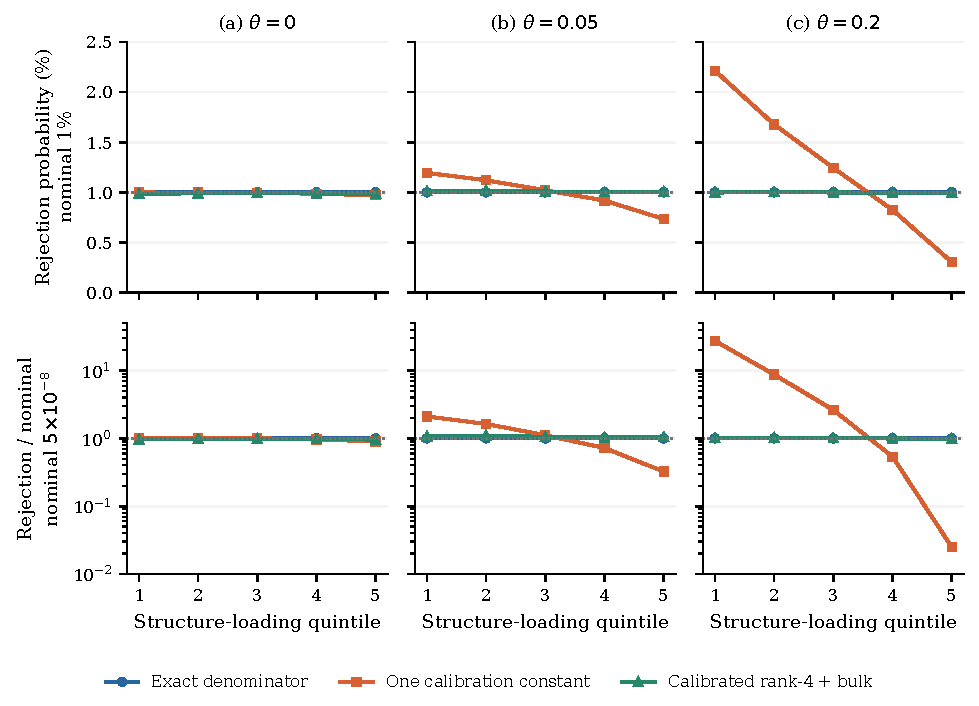
\includegraphics[width=\textwidth]{figures/geometry.pdf}
\caption{Conditional calibration under known covariance. The top row
shows analytic rejection probabilities at a nominal 1\%; the bottom
row shows the ratio of analytic to nominal rejection probability at
$5\times10^{-8}$ on a log scale. Each column is one fixed genotype
panel. Candidate variants are held out from approximation calibration
and ordered by loading on the leading three background eigenvectors.
The spectral method uses four exact eigenvectors and a flat bulk.
Columns share vertical scales. Panels describe denominator geometry, not fitted-covariance or
external-program performance.}
\label{fig:geometry}
\end{figure}

The rank-four correction substantially reduces the loading gradient in
these panels. At $\theta=0.05$, its extreme-quintile probabilities are
1.010\% and 1.005\%; at $\theta=0.20$, they are 0.998\% and 0.992\%.
Its overall analytic rejection ratios at $5\times10^{-8}$ range from
0.97 to 1.06 across the three panels. Held-out root-mean-square relative
denominator-ratio errors are 1.36--1.53\%. This is evidence that the
leading structure directions explain most of the approximation error
in these particular designs. It neither proves that four directions
suffice elsewhere nor tests the accuracy of an estimated leading
subspace.

The empirical rejection fractions agree with their analytic targets
within the script's stated numerical and Monte Carlo tolerance. For the
exact denominator, the overall empirical fractions range from 1.006\%
to 1.007\%, with standard errors approximately 0.010 percentage points.
There is no fitting uncertainty in this comparison: a score with an
exact denominator must have the stipulated marginal law. The simulation
checks the implementation of that construction and quantifies the
sampling variation of the reported summaries.

\subsection{Historical scans show a related pattern, with weaker identification}

The archived strong-structure scan exhibits the same qualitative
gradient (Table~\ref{tab:historical}, Figure~\ref{fig:historical}).
For the scalar infinitesimal implementation, overall $\lgc$ is 0.97,
but the lowest and highest loading quintiles have $\lgc=1.34$ and
0.64, and rejection fractions of 2.45\% and 0.11\% at 1\%. The
historical spectral correction gives 1.14\% and 1.06\% in those
quintiles, close to the dense LOCO results of 1.12\% and 1.11\%.
The KVIK-style implementation retains a pronounced gradient.

\begin{table}[htbp]
\centering\small
\caption{Historical simulated strong-structure panel, six phenotype
replicates. q1 and q5 denote loading quintiles. Rejection fractions are
for the chromosome without generating effects, under the qualifications
in Section~\ref{sec:historicaldesign}. These are archived implementation
results, not a rerun of version 2.0.0.dev1 or reference programs.}
\label{tab:historical}
\begin{tabular}{@{}lccccc@{}}
\toprule
 & & \multicolumn{2}{c}{$\lgc$} & \multicolumn{2}{c}{Rejection (\%)} \\
\cmidrule(lr){3-4}\cmidrule(l){5-6}
Method & $\lgc$, all & q1 & q5 & q1 & q5 \\
\midrule
\tabinput{tables/calibration.tex}
\bottomrule
\end{tabular}
\end{table}

\begin{figure}[htbp]
\centering
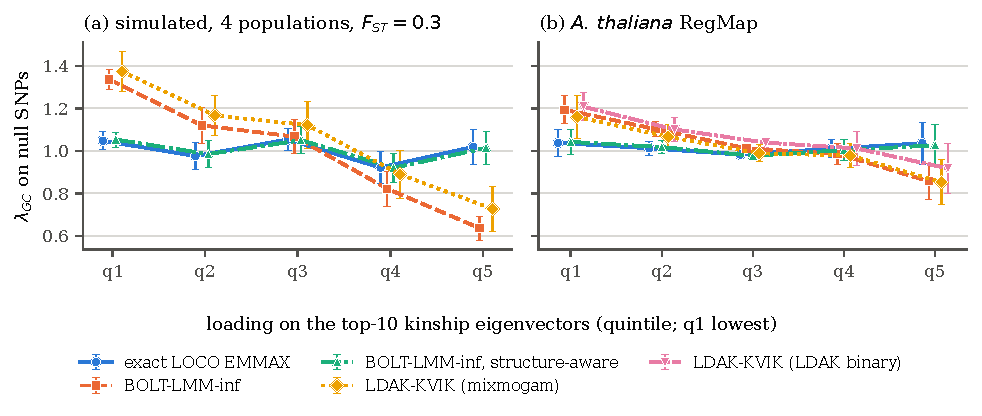
\includegraphics[width=\textwidth]{figures/calibration.pdf}
\caption{Historical strong-structure diagnostics. Points are means over
six phenotype replicates on one fixed genotype panel; bars are 95\%
Student-$t$ intervals for those means. The median statistic and the
nominal 1\% rejection fraction show why reporting only a genome-wide
summary can obscure differences among variant groups. No external
program results are included.}
\label{fig:historical}
\end{figure}

These results are supportive diagnostics, not a second proof of the
mechanism. Variance fitting, sparse generating effects, calibration-marker
selection, and the earlier implementation all contribute to the final
statistics. The new experiment is stronger for identifying denominator
error precisely because it holds those features fixed or removes them.
Conversely, its simplicity limits what it says about the complete scan.
Both evidence types are useful when their roles are kept distinct.

\subsection{Covariance adjustment and environmental adjustment are different}

In the historical S2 stress test, the leading PC predicts deme membership
with squared correlation approximately 0.97. Without kinship adjustment,
QTL-free blocks have $\lgc=11.90$; the mean statistic among variants
with the highest environmental loading is 63.24. Dense LOCO reduces
these summaries to 1.24 and 2.27, but substantial residual structure
remains (Table~\ref{tab:s2}, Figure~\ref{fig:s2}). Including PC1 reduces
them further to 1.09 and 1.13. The corresponding all-variant $\lgc$
falls from 1.27 to 1.11. The residual is reduced, not demonstrably
eliminated.

\begin{table}[htbp]
\centering\small
\caption{Historical S2 environmental stress test, means over three seeds.
Loading refers to squared correlation with the deme exposure. Detection
counts are significant QTL-free blocks, not false positives under a
strict null; these blocks also contain polygenic background effects.
Power is the fraction of designated QTL-containing loci detected under
the archived Bonferroni rule.}
\label{tab:s2}
\begin{tabular}{@{}lccccc@{}}
\toprule
 & & \multicolumn{2}{c}{Mean $\chi^2$} & QTL-free & Locus \\
\cmidrule(lr){3-4}
Method & $\lgc$, QTL-free & Bottom half & Top 1\% & detections & power \\
\midrule
\tabinput{tables/s2.tex}
\bottomrule
\end{tabular}
\end{table}

\begin{figure}[htbp]
\centering
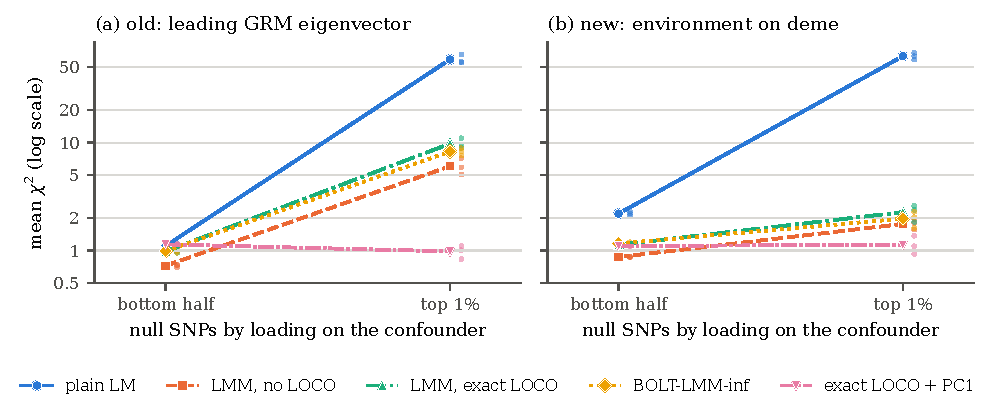
\includegraphics[width=.84\textwidth]{figures/s2_loading.pdf}
\caption{Historical S2 statistics by environmental loading in QTL-free
blocks. Large points and lines show means; small points show the three
simulation seeds. A logarithmic vertical axis accommodates the large
unadjusted mean. PC adjustment reduces the observed gradient, but the
polygenic background and small replicate count prevent a strict-null
calibration claim.}
\label{fig:s2}
\end{figure}

The non-LOCO scan has all-variant $\lgc=0.98$ and QTL-free $\lgc=0.96$,
yet its upper-loading mean remains 1.77 and its locus power is lower
than LOCO's (0.13 versus 0.20). Apparent aggregate calibration is
therefore compatible with both residual environmental structure and
signal attenuation. These data do not identify their separate causal
contributions; a factorial simulation holding the mean and covariance
mechanisms apart is needed.

A related interpretation problem appears in S1 and S3. Replacing fixed
200-marker intervals with LD-aware boundaries reduces the number of
QTL-free detections. In the recorded paired checks, dense LOCO's mean
count changes from 1.33 to zero across three S1 seeds; the single paired
S3 check changes from 17 to 11. This is consistent with
large-QTL signal crossing arbitrary boundaries. It does not establish
that every remaining detection is an error: the background is polygenic,
and alternative block definitions also change the unit of discovery.
Methods for constructing approximately independent LD blocks are useful
here \citep{berisa2016,prive2022}, but evaluation must still define which
biological or statistical null a ``false locus'' is meant to represent.

\subsection{Correctness and computational evidence}
\label{sec:computation}

The current review recorded 117 passing local tests. A separate installed
wheel check on Python 3.10 with NumPy 1.26.4 and SciPy 1.11.4 passed
71 tests, with five skips for unavailable optional HDF5/plotting
components. These checks include independent numerical references and
reproductions of specific defects. The corrected contracts cover PLINK
coding, sample alignment and allele counts, BLUP scaling, variance
fitting, weighted kinships, window complements, permutation geometry,
and effect/standard-error export. Passing them supports those contracts;
it cannot substitute for an end-to-end calibration study.

One allocation change has a directly recorded before/after comparison.
For 800 samples, 1,000 markers, ten LOCO groups, and 80 right-hand sides,
five warm matrix-product repetitions gave identical output arrays.
The measured peak allocation fell from 7,235,824 to 2,625,120 bytes,
a 64\% reduction. This measurement uses Python allocation tracing and
excludes the pre-existing genotype cache and native BLAS allocations;
it is not whole-process peak resident memory. The short timings do not
support a general runtime-speedup claim.

Older timing archives establish why batching and streaming are useful,
but not current competitive performance. One internal comparison
recorded 0.27 seconds for a batched EMMAX scan versus 33.7 seconds for
a per-variant least-squares reference at $n=2,000$, $m=10,000$ (about
123-fold). Historical S3 times were 221 seconds for 25-group dense
LOCO and 18 seconds for the infinitesimal two-step path; a 2.7-second
non-LOCO scan excluded its preceding fit. These workloads differ in
both statistical procedure and accounted work. They were measured on
a development laptop under concurrent activity, not a controlled
cross-program benchmark.

At $n=10,000$, a historical stochastic-Lanczos fit obtained
$\delta=0.91724$ versus 0.91639 for a full fit, a 0.09\% difference in
one case. That agreement concerns one nuisance estimate. A historical
scan based on a truncated spectrum still produced $\lgc=1.30$, versus
0.85 for the full non-LOCO scan. Neither value establishes nominal
calibration in that signal-containing simulation. Accurate likelihood
approximation, accurate association denominators, and calibrated tests
are separate requirements.

\FloatBarrier
\section{Discussion}

\subsection{The central distinction is between geometry and inference}

Equation~\eqref{eq:spectrum} explains the observed conditional gradient
without invoking a software bug: covariance precision weights variant
directions differently. Scalar calibration discards that distinction.
The new experiment shows that restoring a few leading directions can
substantially reduce the error when population structure is concentrated
in those directions and the remaining spectrum is comparatively benign.
It also shows why a good average rejection fraction is insufficient.

The result has a deliberately narrow scope. The leading subspace is
known exactly, the covariance is fixed, genotypes contain no local LD,
and the tested statistic is linear in a Gaussian phenotype before
squaring. Estimated covariance, approximate eigenvectors, rare-allele
sampling, nonlinear shrinkage, and phenotype-dependent selection all
introduce questions not answered by the conditional calculation. The
new results justify further evaluation of the spectral correction;
they do not justify treating it as a generally calibrated replacement
for established GWAS procedures.

\subsection{Prediction accuracy and test validity need separate targets}

A flexible polygenic predictor can reduce residual variance and thereby
improve association power. Yet changing the predictor also changes the
null distribution of a test based on its residuals. Calibration inherited
from an infinitesimal model may not survive a nonlinear prior, tuning
selection, or incomplete optimization. LD Score regression provides a
framework for separating components of genome-wide inflation under its
assumptions \citep{bulikSullivan2015}; an intercept-based rescaling is
not a per-variant guarantee in an arbitrary structured panel.

The same separation applies to reported prediction performance. An
internally tuned or in-sample BLUP is not a prospective prediction
validation. Any future prediction claim needs a held-out sample design
that respects family relationships, ancestry, and the intended target
population. A model can improve prediction while leaving a poorly
calibrated association statistic, and a calibrated test can sacrifice
power through an unsuitable background model.

\subsection{The historical evidence changes the questions, not the standard of proof}

The environmental experiment illustrates the noncentral mean term in
Equation~\eqref{eq:noncentral}. An exposure generated from deme membership
is causally external to the candidate variants in the simulation, but
it is not statistically independent of them. Calling it independent
would remove the very confounding mechanism being studied. A PC defined
from the tested genotypes is also a legitimate mathematical stress axis,
but answers a different question from a separately generated exposure.
Future studies should include both with clearly stated causal and
statistical interpretations.

Similarly, a locus label is a scientific choice. A block without a large
QTL can tag a QTL across its boundary or contain its own small generating
effects. Counting all such discoveries as false positives confounds
localization, power to detect diffuse signal, and test calibration.
The report therefore keeps strict-null experiments separate from
QTL-free-block diagnostics. Real-data significance counts cannot resolve
this ambiguity without additional validation.

\subsection{Limitations and intended use}

The current contribution is strongest as a transparent research
implementation and a framework for controlled comparisons. The new
study contains three small fixed panels, while the broader archived
simulations have three or six replicates and predate important fixes.
No valid matched-input external comparison is retained. There is no
new validation in human multi-ancestry cohorts, no demonstrated
biobank-scale resource profile, and no validation for imputed dosages
or strongly imbalanced binary traits. The latter require attention to
the likelihood and tail approximation, as illustrated by SAIGE's
logistic mixed-model and saddlepoint approach \citep{zhou2018}.

The package exposes useful building blocks, but its multiple modes
should not be presented as interchangeable. Dense plug-in tests,
iterative infinitesimal tests, and nonlinear two-step heuristics differ
in what is approximated. Reporting the mode, grouping, covariance
estimation, convergence diagnostics, and genotype definition is necessary
to make a result interpretable. The most productive next step is to
reduce the gap between those explicit contracts and independently
validated end-to-end behaviour.

\section{Future research: hypotheses and decisive experiments}
\label{sec:future}

The following directions are proposed work, not completed validation.
Their order reflects dependence: reliable input identity and reproducible
reference comparisons are prerequisites for interpreting a new method's
power or speed. Each direction has a hypothesis and a result that could
force it to be revised.

\subsection{Priority 1: establish a matched-input reference benchmark}

\textbf{Question.} After input handling and nuisance definitions are
matched, do the local implementations reproduce an independent Gaussian
reference, and which differences from external programs remain?

The first benchmark should export one validated genotype matrix and
read it back independently, checking individual hard calls, missingness,
sample order, allele orientation, and variant filters before any
phenotype analysis. A frozen manifest should include the marker set,
covariates, phenotype, LOCO map, software versions, commands, and resource
limits. Dense known-covariance and fitted-covariance cases should be
separate. Comparisons with reference BOLT-LMM, LDAK-KVIK, REGENIE, and
Quickdraws should document differences in model and default preprocessing
rather than assume they implement the same test.

\textbf{Decision criterion.} Numerical discrepancies under an identical
Gaussian model must be explained at the effect, standard-error,
variance-component, and statistic levels before aggregate concordance
is accepted. A flat loading gradient in a reference program where the
local approximation shows one would restrict the claim to that local
procedure. More discoveries alone would not establish better calibration
or power. The invalid archived export must not be reused as the matched
input.

\subsection{Priority 2: test calibration independently of adaptive choices}

\textbf{Hypothesis.} An approximation selected on calibration markers
retains its claimed accuracy on independent audit markers and independent
genotype panels.

A nested design should choose spectral width and scaling using one set
of markers and reserve another for evaluation. For LD-containing data,
hold out whole blocks where feasible, because random marker splits can
make an audit nearly redundant with training. If phenotype-dependent
selection is retained, repeat the entire selection and fitting procedure
for every null phenotype. Prespecified strata should include frequency,
missingness, LD score, ancestry loading, kinship leverage, and their
most relevant intersections. Strict-null traits should first be drawn
from a known covariance; fitted-covariance experiments should then add
variance estimation as a separate factor.

\textbf{Decision criterion.} Before running the study, specify acceptable
relative rejection error at each threshold and use uncertainty intervals
across independent phenotype and genotype replicates. A possible initial
criterion is a rejection ratio within 0.9--1.1 at $\alpha=0.01$ in every
adequately powered prespecified stratum; it is a proposed tolerance,
not a standard already met here. Genome-wide tails need their own
error budget and either sufficiently large independent simulations or
a justified rare-event method. Bulk calibration or a 3\% training-ratio
spread cannot stand in for that evidence. Persistent failures in an
audited stratum should trigger a more accurate denominator or an explicit
unsupported-case result.

\subsection{Priority 3: replace spectral heuristics with computable error bounds}

\textbf{Hypothesis.} A hybrid method can retain streaming efficiency while
bounding denominator error for difficult variants.

Suppose the omitted eigenvalues are known to lie in $[a,b]$, with
$a+\delta>0$, and let
$s_j=\|\z_j\|^2-\sum_{\ell\leq k}a_{\ell j}^2$.
The exact retained contribution $q_{j,\leq k}$ then yields
\begin{equation}
 q_{j,\leq k}+\frac{s_j}{b+\delta}
 \ \leq\ q_j\ \leq\
 q_{j,\leq k}+\frac{s_j}{a+\delta}.
 \label{eq:tailbound}
\end{equation}
This interval can be propagated through Equation~\eqref{eq:tail},
or through a fixed score numerator, to determine whether an approximation
is adequate at the requested threshold. Variants with wide intervals
could receive additional spectral work or an iterative exact-denominator
solve. Approximate Ritz values alone do not certify the spectrum:
residual bounds and uncertainty in the retained subspace must be
included. Equation~\eqref{eq:tailbound} states a possible mathematical
contract, not an implemented certificate.

Iterative solves offer a complementary bound. For
$A=\K+\delta\I\succeq\delta\I$, approximate solution
$\widehat{\w}$, and residual $\mathbf r=\y-A\widehat{\w}$,
\begin{equation}
 \big|\z_j^\top(A^{-1}\y-\widehat{\w})\big|
 \leq \frac{\|\z_j\|\,\|\mathbf r\|}{\delta}.
 \label{eq:cgbound}
\end{equation}
A corresponding solve with right-hand side $\z_j$ bounds denominator
error. Such bounds may be loose, especially for small $\delta$, but
make the numerical target explicit.

\textbf{Decision criterion.} Compare bounds with dense references on
small problems, then record how often fallback solves are required,
whole-process peak memory, and end-to-end time. The approach is useful
only if the bound is honest and selective enough to save work. Even a
perfect numerical certificate would leave estimated-covariance and
model-misspecification questions unresolved.

\subsection{Priority 4: derive calibration for nonlinear polygenic residuals}

\textbf{Hypothesis.} Mixture and elastic-net residuals need a calibration
that reflects their own response to the phenotype, rather than a
transferred infinitesimal factor.

Start with a sequence of models whose complexity increases: fixed
ridge shrinkage, tuned ridge, a fixed mixture prior, and then jointly
tuned nonlinear models. For each, compare a conditional analytic or
influence-function approximation where available with a parametric
bootstrap that repeats fitting and hyperparameter selection. Sample splitting
or cross-fitting, combined with candidate-region exclusion, may reduce reuse
of information between nuisance fitting and testing, but does not by itself
establish a null law. Null
simulation should include both correctly specified and deliberately
misspecified effect distributions, with convergence tolerances varied
independently of prior choice.

\textbf{Decision criterion.} An apparent power gain is retained only if
it survives equal-calibration comparisons at matched type-I error and
can be separated from incomplete optimization or reuse of the same data
for tuning. Failure of the infinitesimal factor after nonlinear fitting
would support method-specific calibration, not a universal multiplicative
repair. Reference-program comparisons are essential because an error
in a local reimplementation is not a property of the published method.

\subsection{Priority 5: separate mean confounding, covariance error, and localization}

\textbf{Hypothesis.} The benefit and cost of PC adjustment depend on
which part of the data-generating process is misspecified, and apparent
null-locus inflation depends on the discovery unit.

A factorial simulation should vary ancestry-associated exposure from
zero through modest effects to the S2 stress level; covariance fit from
known truth to fitted and misspecified kinships; and fixed covariates
from none to measured exposure and prespecified PCs. Demographic scenarios
should include recent relatives, admixture, unequal ancestry sample sizes,
and LD. Generate some outcomes under a strict null and others under
sparse, polygenic, and ancestry-dependent effects. Report effect bias,
interval coverage, conditional rejection, calibrated power, and
between-ancestry performance. PC count should be chosen without looking
at the final calibration outcome, or its selection repeated within
validation.

For signal-containing traits, distinguish causal-variant recovery,
LD-tagged association, and block-level localization. A QTL-free block
should be called a false discovery only under a null definition that
actually excludes its background and tagging effects. Fixed boundaries,
LD-aware boundaries, and explicitly independent simulated blocks should
be compared on the same underlying genotypes where possible.

\textbf{Decision criterion.} If LOCO is calibrated without PCs at modest
exposure levels, the strong S2 result should remain a stress-test finding.
If PCs reduce bias but also remove genuine ancestry-dependent signal,
that trade-off must be reported instead of optimizing $\lgc$ toward one.
A block method is better only if it improves the stated localization
objective, not merely because relabelling blocks reduces a count.

\subsection{Priority 6: make scale and reproducibility part of method design}

\textbf{Hypothesis.} Packed genotype access, bounded caches, and selective
precision can improve practical scale without changing the statistical
procedure.

Benchmark whole workflows across sample size, marker count, missingness,
number of LOCO groups, and genotype storage backend. Record setup,
variance fitting, prediction, testing, and output time separately,
as well as total wall time, CPU time, and process peak resident memory.
Warm-cache and cold-cache runs should be distinguished. Measure the cost
of diagnostics and fallback calculations, rather than reporting their
benefits against a baseline that omits them. Mixed-precision variants
should be judged by errors in effect estimates, small denominators,
and tail probabilities, not only normwise matrix error.

A useful extension would add a carefully specified continuous-dosage
interface with imputation-quality handling and independent decoding
fixtures. Binary traits require a separate modelling and calibration
programme; simply passing zeros and ones to a Gaussian scan is not the
proposed extension. Prospective prediction, if developed, should use
held-out families or populations and report transportability separately
from association power.

\textbf{Decision criterion.} A scalability claim should identify the
validated data size, hardware, resource limits, and failure boundary.
A speedup is scientifically useful only if the inferential target and
accuracy are preserved. Release artifacts should reproduce a compact
set of known-truth calculations and input round trips before any larger
performance claim is made.

\section*{Data, software, and reproducibility}

The repository is available at
\url{https://github.com/bvilhjal/mixmogam}. This report describes package
version 2.0.0.dev1; the current numerical experiment uses baseline commit
\code{729c8532}. Its self-contained driver is
\code{benchmarks/denominator\_geometry.py}, with results, source snapshot,
and manifest in \code{20261003-manuscript-geometry} beneath
\code{benchmarks/results/}. The review archive is
\code{20261003-critical-review}. Historical inputs retain their original
source snapshots. The excluded external-program archive is also preserved
for provenance; its results are not incorporated into the revised displays.

\code{report/README.md} gives the reproduction commands, exact archive
identities, and evidence map. The figure generator reads recorded results and does not silently
rerun old analyses. The figure and report manifests identify source
hashes; the bibliography metadata records verified DOI identities.
No new human-participant data were collected for this revision. The
new experiment is entirely simulated. Historical RegMap results are
not used to support current performance claims.

\appendix
\section{Useful identities and interpretation checks}
\label{sec:appendix}

\subsection{Whitening explains the known-shape F reference}

Let $L=\Hm^{-1/2}$ and let $Q$ span $L\X$ orthonormally. The whitened
residual phenotype is $\mathbf r=(\I-QQ^\top)L\y$ and the residual
candidate is $\mathbf v_j=(\I-QQ^\top)L\z_j$. Under the known-shape
Gaussian null, the squared projection onto $\mathbf v_j$ and the
remaining residual sum of squares are independent scaled chi-squares
with one and $n-p-1$ degrees of freedom. Their ratio is
Equation~\eqref{eq:f}. When $L$ is estimated from $\y$, this fixed-linear-
transformation argument no longer proves the reference law. It explains
precisely where the plug-in approximation enters.

\subsection{Residual coordinates for permutation}

Choose an $n\times(n-p)$ orthonormal matrix $B$ spanning the complement
of $L\X$. With known Gaussian covariance shape,
\begin{equation}
 \mathbf t=B^\top L\y\sim N(0,\sigma_g^2\I_{n-p}),\qquad
 \Var\{(\I-QQ^\top)L\y\}=\sigma_g^2(\I-QQ^\top).
 \label{eq:permutation}
\end{equation}
The entries of $\mathbf t$ are exchangeable; the $n$ entries of the
projected residual generally are not. A valid residual-coordinate
transformation therefore permutes $\mathbf t$ and maps it back through
$B$, rather than permuting arbitrary sample-coordinate residuals.
The implementation uses orthogonal transformations without storing an
additional full complement matrix in the production path. Estimated
covariance, non-Gaussian errors, and repeated model selection require
separate investigation; algebraic exchangeability under a known model
should not be advertised as an unconditional guarantee.

\subsection{BLUP scale and a marginal Bayes factor}

The genetic conditional mean uses
$\operatorname{Cov}(\mathbf u,\y)=\sigma_g^2\K$ and
$\Var(\y)=\sigma_g^2\Hm$, hence
\begin{equation}
 \widehat{\mathbf u}=\sigma_g^2\K(\sigma_g^2\Hm)^{-1}
 (\y-\X\widehat{\boldsymbol\beta})
 =\K\Hm^{-1}(\y-\X\widehat{\boldsymbol\beta}).
 \label{eq:blup}
\end{equation}
This identity is conditional on fitted parameters when used in the
package. In-sample fitted genetic values do not measure prospective
prediction accuracy.

For a marginal effect estimate $\widehat\alpha$ with sampling variance
$v$, assume $\widehat\alpha\mid\alpha\sim N(\alpha,v)$ and an
alternative prior $\alpha\sim N(0,W)$. Against a point null at zero,
the approximate Bayes factor is
\begin{equation}
 \mathrm{BF}_{10}=\sqrt{\frac{v}{v+W}}
 \exp\left\{\frac{\widehat\alpha^2 W}{2v(v+W)}\right\}.
 \label{eq:abf}
\end{equation}
The prior variance $W$ has the units of the squared effect and must be
chosen explicitly. Posterior odds additionally require prior odds;
normalizing marginal factors across correlated variants does not by
itself yield a multi-variant fine-mapping posterior. The corrected API
therefore no longer presents an RSS-based pseudo-score as a posterior
probability.

\begin{thebibliography}{99}
\raggedright

\bibitem[Abney(2015)]{abney2015}
Abney M (2015). Permutation testing in the presence of polygenic
variation. \emph{Genet Epidemiol} 39(4):249--258.
\href{https://doi.org/10.1002/gepi.21893}{doi:10.1002/gepi.21893}


\bibitem[Baumdicker et~al.(2022)]{baumdicker2022}
Baumdicker F, Bisschop G, Goldstein D, et~al. (2022). Efficient ancestry
and mutation simulation with msprime 1.0. \emph{Genetics} 220(3):iyab229.
\href{https://doi.org/10.1093/genetics/iyab229}{doi:10.1093/genetics/iyab229}

\bibitem[Berisa and Pickrell(2016)]{berisa2016}
Berisa T, Pickrell JK (2016). Approximately independent linkage
disequilibrium blocks in human populations. \emph{Bioinformatics}
32(2):283--285.
\href{https://doi.org/10.1093/bioinformatics/btv546}{doi:10.1093/bioinformatics/btv546}

\bibitem[Bhatia et~al.(2013)]{bhatia2013}
Bhatia G, Patterson N, Sankararaman S, Price AL (2013). Estimating and
interpreting $F_{ST}$: the impact of rare variants. \emph{Genome Res}
23(9):1514--1521.
\href{https://doi.org/10.1101/gr.154831.113}{doi:10.1101/gr.154831.113}

\bibitem[Bulik-Sullivan et~al.(2015)]{bulikSullivan2015}
Bulik-Sullivan BK, Loh P-R, Finucane HK, et~al. (2015). LD Score
regression distinguishes confounding from polygenicity in genome-wide
association studies. \emph{Nat Genet} 47(3):291--295.
\href{https://doi.org/10.1038/ng.3211}{doi:10.1038/ng.3211}

\bibitem[Hof and Speed(2025)]{hof2025}
Hof JP, Speed D (2025). LDAK-KVIK performs fast and powerful mixed-model
association analysis of quantitative and binary phenotypes.
\emph{Nat Genet} 57(9):2116--2123.
\href{https://doi.org/10.1038/s41588-025-02286-z}{doi:10.1038/s41588-025-02286-z}

\bibitem[Horton et~al.(2012)]{horton2012}
Horton MW, Hancock AM, Huang YS, et~al. (2012). Genome-wide patterns of
genetic variation in worldwide \emph{Arabidopsis thaliana} accessions
from the RegMap panel. \emph{Nat Genet} 44(2):212--216.
\href{https://doi.org/10.1038/ng.1042}{doi:10.1038/ng.1042}

\bibitem[Kang et~al.(2008)]{kang2008}
Kang HM, Zaitlen NA, Wade CM, et~al. (2008). Efficient control of
population structure in model organism association mapping.
\emph{Genetics} 178(3):1709--1723.
\href{https://doi.org/10.1534/genetics.107.080101}{doi:10.1534/genetics.107.080101}

\bibitem[Kang et~al.(2010)]{kang2010}
Kang HM, Sul JH, Service SK, et~al. (2010). Variance component model to
account for sample structure in genome-wide association studies.
\emph{Nat Genet} 42(4):348--354.
\href{https://doi.org/10.1038/ng.548}{doi:10.1038/ng.548}

\bibitem[Kelleher et~al.(2016)]{kelleher2016}
Kelleher J, Etheridge AM, McVean G (2016). Efficient coalescent
simulation and genealogical analysis for large sample sizes.
\emph{PLoS Comput Biol} 12(5):e1004842.
\href{https://doi.org/10.1371/journal.pcbi.1004842}{doi:10.1371/journal.pcbi.1004842}

\bibitem[Lippert et~al.(2011)]{lippert2011}
Lippert C, Listgarten J, Liu Y, et~al. (2011). FaST linear mixed models
for genome-wide association studies. \emph{Nat Methods} 8(10):833--835.
\href{https://doi.org/10.1038/nmeth.1681}{doi:10.1038/nmeth.1681}

\bibitem[Listgarten et~al.(2012)]{listgarten2012}
Listgarten J, Lippert C, Kadie CM, et~al. (2012). Improved linear mixed
models for genome-wide association studies. \emph{Nat Methods}
9(6):525--526.
\href{https://doi.org/10.1038/nmeth.2037}{doi:10.1038/nmeth.2037}

\bibitem[Loh et~al.(2015)]{loh2015}
Loh P-R, Tucker G, Bulik-Sullivan BK, et~al. (2015). Efficient Bayesian
mixed-model analysis increases association power in large cohorts.
\emph{Nat Genet} 47(3):284--290.
\href{https://doi.org/10.1038/ng.3190}{doi:10.1038/ng.3190}


\bibitem[Loya et~al.(2025)]{loya2025}
Loya H, Kalantzis G, Cooper F, Palamara PF (2025). A scalable
variational inference approach for increased mixed-model association
power. \emph{Nat Genet} 57(2):461--468.
\href{https://doi.org/10.1038/s41588-024-02044-7}{doi:10.1038/s41588-024-02044-7}

\bibitem[Mbatchou et~al.(2021)]{mbatchou2021}
Mbatchou J, Barnard L, Backman J, et~al. (2021). Computationally
efficient whole-genome regression for quantitative and binary traits.
\emph{Nat Genet} 53(7):1097--1103.
\href{https://doi.org/10.1038/s41588-021-00870-7}{doi:10.1038/s41588-021-00870-7}

\bibitem[Price et~al.(2006)]{price2006}
Price AL, Patterson NJ, Plenge RM, et~al. (2006). Principal components
analysis corrects for stratification in genome-wide association
studies. \emph{Nat Genet} 38(8):904--909.
\href{https://doi.org/10.1038/ng1847}{doi:10.1038/ng1847}

\bibitem[Price et~al.(2010)]{price2010}
Price AL, Zaitlen NA, Reich D, Patterson N (2010). New approaches to
population stratification in genome-wide association studies.
\emph{Nat Rev Genet} 11(7):459--463.
\href{https://doi.org/10.1038/nrg2813}{doi:10.1038/nrg2813}

\bibitem[Priv\'e(2022)]{prive2022}
Priv\'e F (2022). Optimal linkage disequilibrium splitting.
\emph{Bioinformatics} 38(1):255--256.
\href{https://doi.org/10.1093/bioinformatics/btab519}{doi:10.1093/bioinformatics/btab519}

\bibitem[Segura et~al.(2012)]{segura2012}
Segura V, Vilhj\'almsson BJ, Platt A, et~al. (2012). An efficient
multi-locus mixed-model approach for genome-wide association studies in
structured populations. \emph{Nat Genet} 44(7):825--830.
\href{https://doi.org/10.1038/ng.2314}{doi:10.1038/ng.2314}

\bibitem[Sul et~al.(2018)]{sul2018}
Sul JH, Martin LS, Eskin E (2018). Population structure in genetic
studies: confounding factors and mixed models. \emph{PLoS Genet}
14(12):e1007309.
\href{https://doi.org/10.1371/journal.pgen.1007309}{doi:10.1371/journal.pgen.1007309}

\bibitem[Vilhj\'almsson and Nordborg(2013)]{vilhjalmsson2013}
Vilhj\'almsson BJ, Nordborg M (2013). The nature of confounding in
genome-wide association studies. \emph{Nat Rev Genet} 14(1):1--2.
\href{https://doi.org/10.1038/nrg3382}{doi:10.1038/nrg3382}


\bibitem[Wakefield(2009)]{wakefield2009}
Wakefield J (2009). Bayes factors for genome-wide association studies:
comparison with P-values. \emph{Genet Epidemiol} 33(1):79--86.
\href{https://doi.org/10.1002/gepi.20359}{doi:10.1002/gepi.20359}

\bibitem[Yang et~al.(2010)]{yang2010}
Yang J, Benyamin B, McEvoy BP, et~al. (2010). Common SNPs explain a
large proportion of the heritability for human height. \emph{Nat Genet}
42(7):565--569.
\href{https://doi.org/10.1038/ng.608}{doi:10.1038/ng.608}

\bibitem[Yang et~al.(2014)]{yang2014}
Yang J, Zaitlen NA, Goddard ME, Visscher PM, Price AL (2014). Advantages
and pitfalls in the application of mixed-model association methods.
\emph{Nat Genet} 46(2):100--106.
\href{https://doi.org/10.1038/ng.2876}{doi:10.1038/ng.2876}

\bibitem[Zhou and Stephens(2012)]{zhou2012}
Zhou X, Stephens M (2012). Genome-wide efficient mixed-model analysis
for association studies. \emph{Nat Genet} 44(7):821--824.
\href{https://doi.org/10.1038/ng.2310}{doi:10.1038/ng.2310}


\bibitem[Zhou et~al.(2018)]{zhou2018}
Zhou W, Nielsen JB, Fritsche LG, et~al. (2018). Efficiently controlling
for case-control imbalance and sample relatedness in large-scale
genetic association studies. \emph{Nat Genet} 50(9):1335--1341.
\href{https://doi.org/10.1038/s41588-018-0184-y}{doi:10.1038/s41588-018-0184-y}

\end{thebibliography}

\end{document}
